% Drawing 80/01-9 -- folder 80, batch 01, archive page 18 (PDF page 19).
% Transcription: dans la marge gauche, en regard du paragraphe barré, un petit croquis : un contour fermé (une sphère) et, à l'intérieur, deux arcs qui se coupent en deux points marqués, en haut et en bas, un troisième arc en tirets entre eux ; à gauche, un « ? »
% Kind: sphere with two arcs meeting at two antipodal points. Method 2 (schematic redraw from the facsimile). Status: ok.
% Notes: Ink. Closed outline; two arcs from the upper marked point to the lower one, forming an oval; a dashed arc between the same two points and a short dashed arc near the top right; the question mark at the left. The long stroke that crosses the sketch at the left is one of the strokes striking out the paragraph and is not drawn. Redrawn 2026-11-12 (issue 128): to check again.
% Coordinates: 1 unit = 1 mm = 1/100 of the crop width (bbox in page fractions: [0.09, 0.6, 0.33, 0.69]).
% Redrawn by Claude (claude-fable-5-2), issue #128, 2026-11-12; not checked by a human; not compiled (no TeX in the session).
% Rights: reproduces part of the work -- behind RENDER_TRANSCRIPTS, never published by itself.
\documentclass[tikz,border=3pt]{standalone}
\usepackage{amsmath,amssymb}
\usetikzlibrary{patterns,arrows.meta}
\tikzset{pencil/.style={black!45}, struck/.style={black!35}, mpt/.style={circle,draw,inner sep=1.3pt}, pt/.style={circle,fill,inner sep=0.9pt}, opt/.style={circle,draw,fill=white,inner sep=1.1pt}}
\begin{document}
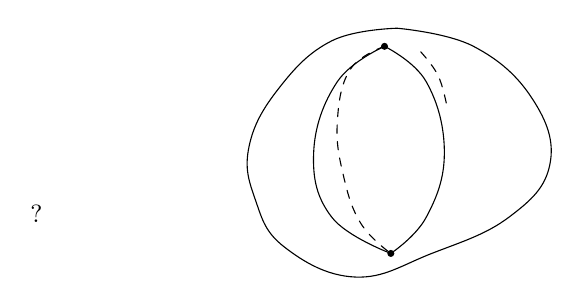
\begin{tikzpicture}[x=1mm,y=1mm,line cap=round,line join=round,font=\scriptsize]
\draw plot[smooth, tension=0.7] coordinates {(67.8,-11.2) (77.5,-13.5) (85,-20.2) (87.2,-28.5) (82,-35.2) (72.2,-39.8) (62.5,-42.8) (53.5,-39) (49.8,-33) (49,-26.2) (52.8,-18.8) (59.5,-12.8) (67.8,-11.2)};
\draw plot[smooth, tension=0.7] coordinates {(66.2,-13.5) (60.2,-18) (57.2,-27) (59.5,-35.2) (67,-39.8)};
\draw plot[smooth, tension=0.7] coordinates {(66.2,-13.5) (71.5,-18) (73.8,-27) (71.5,-35.2) (67,-39.8)};
\draw[dashed] plot[smooth, tension=0.7] coordinates {(66.2,-13.5) (61.8,-16.5) (60.2,-23.2) (61,-30) (63.2,-36) (67,-39.8)};
\draw[dashed] plot[smooth, tension=0.7] coordinates {(70.8,-14.2) (73,-17.2) (74.1,-21)};
\node[pt] at (66.2,-13.5) {};
\node[pt] at (67,-39.8) {};
\node[inner sep=1pt] at (22,-34.8) {\small ?};
\end{tikzpicture}
\end{document}
